% Created 2016-09-14 三 20:25
\documentclass[11pt]{ctexart}
\usepackage[utf8]{inputenc}
\usepackage[T1]{fontenc}
\usepackage{fixltx2e}
\usepackage{graphicx}
\usepackage{longtable}
\usepackage{float}
\usepackage{wrapfig}
\usepackage{rotating}
\usepackage[normalem]{ulem}
\usepackage{amsmath}
\usepackage{textcomp}
\usepackage{marvosym}
\usepackage{wasysym}
\usepackage{amssymb}
\usepackage[CJKbookmarks,colorlinks,linkcolor=black]{hyperref}
\usepackage{graphicx}
\usepackage{wrapfig}
\tolerance=1000
\author{pal}
\date{\today}
\title{resume}
\hypersetup{
  pdfkeywords={},
  pdfsubject={},
  pdfcreator={Emacs 25.1.1 (Org mode 8.2.10)}}
\begin{document}

\maketitle
\tableofcontents

\section{个人简历}
\label{sec-1}
\subsection{基本信息}
\label{sec-1-1}

\begin{wrapfigure}{r}{2in}
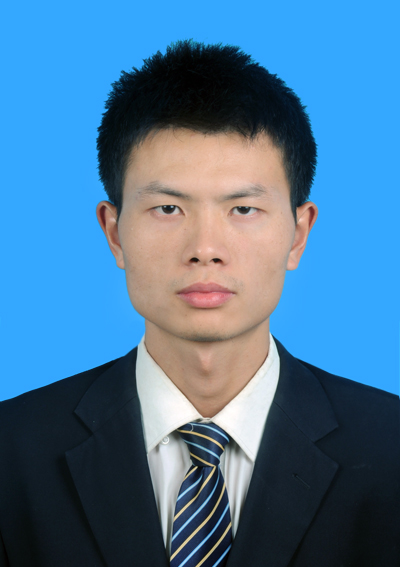
\includegraphics[height=1.2in]{portrait}\
\end{wrapfigure}
\noindent{姓名:胡月恒}\\
性别:男\\
应聘岗位:Java软件工程师\\
学历:硕士(应届毕业生)\\
手机:13323833820\\
邮箱:palagend@163.com\\
出生年月:1990-10-09\\
专业:测试计量技术及仪器(嵌入式方向)\\



\subsection{技能描述}
\label{sec-1-2}
\subsubsection{Java}
\label{sec-1-2-1}
\begin{enumerate}
\item java语言基础:OOP思想,设计模式,文件IO,socket编程,多线程,JDBC,java反射机制;
\item web基础:http,servlet,jsp;
\item 使用过的框架:Spring,Hibernate,JPA;
\item 熟悉的开发工具:Atom,Eclipse,Tomcat,Jboss,Maven
\end{enumerate}
\subsubsection{Linux}
\label{sec-1-2-2}
\begin{enumerate}
\item 熟悉的发行版:红帽系列
\item 脚本编程:bash脚本编程
\item 编辑器:vim,emacs,atom
\item 编译工具:gcc
\end{enumerate}
\subsubsection{数据库}
\label{sec-1-2-3}
\begin{enumerate}
\item 基础:SQL
\item MySQL(MariaDB):复杂查询,数据库备份,数据库范式
\item Oracle:oracle工作原理
\end{enumerate}
\subsubsection{其他}
\label{sec-1-2-4}
\begin{enumerate}
\item Javascript,Python,Php;
\item jQuery,Angular,easyui;
\item Node.js;
\item Android
\end{enumerate}
\subsection{校内实践}
\label{sec-1-3}
\begin{enumerate}
\item 乒乓球赛;
\item 组织专业同学聚会;
\item 参加迎新晚会;
\item 踊跃参与入党积极分子培训班;
\item 在河南有线实习期间参与认证系统的维护和二次开发;
\end{enumerate}
\subsection{项目经验}
\label{sec-1-4}
\subsubsection{河南有线网络接入认证系统}
\label{sec-1-4-1}
\textbf{项目描述}:这是我实习期间接受的第一个工作任务,为认证系统添加radius认证功能.这是一个比较老的项目,用的是EJB和jboss技术,框架采用的是struts.\\
\textbf{项目经验}:第一次对旧项目做维护,感觉真的很棘手,因为之前并没有关注EJB和jboss,对struts这一过时的技术更是直接忽略;但是既然接手了任务,也只能
硬着头皮往前冲了.我先是花了一个晚上的时间恶补了EJB和jboss的知识,然后写了一些小demo练练手熟悉熟悉.等了解RMI的工作原理,jboss和tomcat之
间的关系之后,思路就清晰多了;接下来是阅读项目源码,理清逻辑结构(代码没有文档,真的很痛苦,花了不少时间).通过与业务人员的沟通,了解RADIUS认证的业务流程
,然后就是写代码了,根据OSS传过来的指令,对RADIUS数据库作相应的CRUD操作(小case).回过头来想想这整个过程,大多时间是用在学习消化新知识上面了
,而写代码本身并没有占用太多时间.这种经验,在课堂上肯定是学不来的.
\subsubsection{河南有线网络分销系统二期}
\label{sec-1-4-2}
\textbf{涉及的技术}:Spring, Hibernate, EasyUI, MySQL\\
\textbf{开发工具和平台}:MyEclipse, SVN, Atom\\
\textbf{项目描述}:这是一个web项目,与河南有线合作的各级代理分销商可以通过这个平台,给用户缴纳上网费\\
\textbf{项目经验}:说实话,这个项目的开发体验并不好,但也吸取了不少反面教训.首先是前期需求都还不确定的情况下,就要求马上开工,而且只给一个月的时间,要实现缴费,权限分配,产品宣传,报表打印,库存管理,界面还要美观大方,稳定可靠,希望开发完了马上上线,然而开发人员总共就两个.既要短平快,又要大而全,这倒还不算什么,与银行接口协议都还没谈好的情况下,就让我自己先定接口,程序先写着,说如果需求有变化,再改过来就是了(真的好无语).各部门之间扯皮,数据结构混乱,文档不全或几乎没有,有时候只能通过变量名揣测大概意思.另外进度还催得很紧,
为了赶工期,我前端选用了一个Ace模板作为框架,一些控件直接套用EasyUI,因为催得紧,人手又不够,代码大多是只求运行通过,优化比较少.一个月下来勉强完成了任务,但是整体的开发体验真的不好,虽然能运行,但是代码写的很乱.通过这一次糟糕的开发体验,我明白了,软件开发不只是纯技术的问题,软件的管理也是相当重要的,如果管理不到位,倚天剑也会被用成了砍柴刀.
\subsubsection{基于百度地图SDK的手机定位App}
\label{sec-1-4-3}
\textbf{涉及的技术}:Baidu LBS,Android,java\\
\textbf{开发工具和平台}:Android Studio,android手机\\
\textbf{项目描述}:这是我作毕业论文期间需要采集车辆行驶数据而编写的一个手机端定位数据采集App,功能比较简单,就是采集驾驶员行车时的定位数据并保存到本地文件中,供后期分析处理;\\
\textbf{项目收获}:本人主要学的是java,而安卓与java有着千丝万缕的亲缘关系,我也就尝试着做了一个android app.从android开发环境的搭建,到百度SDK的学习,从程序设计,在到app发布.整个过程都是自力更生,摸石头过河走过来的.虽然是半道出家搞android,但整个过程让我对android系统有了深入的了解.如果将来有转到android开发的需求应该不会太辛苦.\\
\subsubsection{博客发布系统}
\label{sec-1-4-4}
经过之前糟糕的开发体验,我也找了自身的原因,技能还是不扎实,面对快节奏时才会手忙脚乱.于是抽了一段时间学习Spring的源码,并结合设计模式的书籍理解大神的设计艺术,但是总有点空空的感觉;于是我想到做一个玩具项目当做自己的练兵场,尽量把平时学到的新知识运用到这个项目中以巩固自己.项目托管在Github上(\href{http://github.com/palagend/luna}{博客发布系统}),git的版本控制日志可以当做自己的学习笔记.
\subsection{所获奖项或证书}
\label{sec-1-5}
高级软件工程师;
高级数据库管理工程师;
系统分析师;
英语六级;
全国大学生电子设计大赛一等奖;
研究生学业奖学金;
优秀班干部;
驾驶证;
\subsection{兴趣爱好}
\label{sec-1-6}
捣鼓linux,看博客,读书,听歌,爱运动
\subsection{自我评价}
\label{sec-1-7}
\begin{enumerate}
\item 自学能力强. 当我面对陌生的新技术时,不会束手无策,而是通过上网搜索或是翻阅书籍自主学习新知识;在检索信息的过程中注重检索技巧, 首先粗略搜索,逛逛论坛看看博客,获取感性上的认识;然后,逐步缩小搜索范围,再阅读官方英文文档深入研究,直到get新技能.\\
\item 专注. 当我想做成一件事时,会自动屏蔽外界的干扰,整个脑子都被自己所想的事情给占据了,这样的发呆状态甚至会被朋友误以为抑郁了.\\
\item "悲观"的豁达者. 这个"悲观"的意思不是指通常意义上的那种对生活不抱希望的意思.真正的意思是,我不大相信生活会有什么奇迹发生,对任何事情都是做好最坏的打算,然后想出尽可能多的应对方案.豁达是指,对木已成舟的过往琐事不去懊悔计较,免得让自己心烦.总之,大概就是"听天命,尽人事"的意思吧.
\end{enumerate}
% Emacs 25.1.1 (Org mode 8.2.10)
\end{document}